\chapter{Stand van zaken}
\label{ch:stand-van-zaken}

% Tip: Begin elk hoofdstuk met een paragraaf inleiding die beschrijft hoe
% dit hoofdstuk past binnen het geheel van de bachelorproef. Geef in het
% bijzonder aan wat de link is met het vorige en volgende hoofdstuk.

% Pas na deze inleidende paragraaf komt de eerste sectiehoofding.

% TODO CONTENT Inleiding
% TODO Verwijderen template text
Door de recente opkomst van nieuwe virtual reality applicaties denken veel mensen dat VR een nieuwe technologie is. Alhoewel dat de exacte oorsprong van VR moeilijk te achterhalen is omdat er geen vaste definitie van bestaat, kan één van de eerste commerciële toepassingen gevonden worden in 1939, namelijk de View-Master. Gebruikers konden door dit apparaat kijken om zo full-screen panorama's te zien van locaties in de wereld. Een ander voorbeeld is de Sensorama van (INSERT CITE). Deze machine had de mogelijkheid om een video af te spelen en ondertussen de zintuigen van de gebruiker te stimuleren. Dit was mogelijk door geuren, wind en bewegingen na te bootsen.
\begin{figure}
    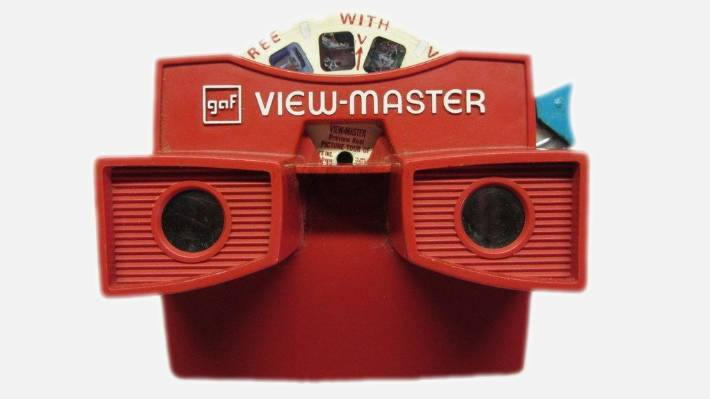
\includegraphics[width=\linewidth]{viewmaster.jpg}
    \caption{De View-Master, uitgebracht in 1939}
    \label{fig:viewmaster}
\end{figure}

\begin{figure}
    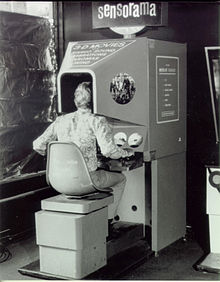
\includegraphics[width=\linewidth]{sensorama.jpg}
    \caption{De Sensorama}
    \label{fig:sensorama}
\end{figure}

\section{Teleprescence}
Tijdens het gebruik van een VR applicatie is gebruiker aanwezig in 2 "werelden" tegelijk, teleprescence is dus dat de gebruiker zich meer aanwezig voelt in de virtuele wereld dan de fysieke wereld.
Een grote fout die veel mensen maken is Virtual Reality koppelen aan hardware terwijl dit veel meer dan dit is \autocite{Steuer1992}.
Perceptie van automatische en gecontrolleerde mentale processen

Teleprescence komt niet alleen voor bij VR maar bij elke applicatie waarbij er gebruik wordt gemaakt van een communicatie medium. Dit communicatie medium is niet alleen digitaal ook fysieke zaken zoals kranten kan je het gevoel geven dat je er echt 'aanwezig' bent, mensen ervaren dit soms als rillingen wanneer ze bijvoorbeeld iets choquerend lezen. 
Een groot verschil tussen VR en de andere mediums waarbij teleprescence in meespeelt is dat bij VR de gebruiker beide zender en ontvanger is. Hij zal acties versturen naar de virtuele wereld en beelden terug krijgen op basis van zijn acties.
Aan de hand van deze definitie kunnen we dus afleiden dat zelfs 360 graden video's ook als VR tellen. Dit is omdat de beelden die de gebruiker te zien krijgt afhangen van de draaihoek hoe hij kijkt naar het scherm zelfs telefoneren kan men eigenlijk zien als VR \autocite{Steuer1992}.
Omdat deze definitie van VR heel ruim is beperkt deze bachelorproef zich tot de technologieën die gebruiken maken van een gyroscoop of andere sensoren om zo een betere ervaring te geven.

% TODO TRANSLATE Immersive
Om het niveau van teleprescence te verhogen bij de gebruiker moet er rekening worden gehouden met 2 variabelen: de immersive / echtheid en de interactiviteit van de applicatie \autocite{Steuer1992}.
De belangrijkste factor die de echtheid van een applicatie verhoogt is de stimulatie van de zintuigen. Wanneer de gebruiker bijvoorbeeld echt de wind en het water voelt terwijl hij in een virtuele regen staat zal hij misschien meer geneigd zijn om de virtuele wereld als echt te gaan ervaren \autocite{Steuer1992}. De invloed van deze externe factoren kan afhangen van gebruiker tot gebruiker, sommige gebruikers staan hier meer voor open en zullen zich sneller ondergedompeld voelen in de ervaring dan anderen.
Interactiviteit kan op verschillende manieren worden verhoogd, de manier waarop zal vaak afhangen van de gekozen technologie. Wanneer een HMD (Head Mounted Display) wordt gebruikt heeft de gebruiker beide handen vrij om acties te doen. Deze acties kunnen dan gebeuren door het herkennen van de lichaamsdelen of door externe controllers.
Met het herkennen van de lichaamsdelen wordt er bedoeld dat de software effectief het lichaamsdeel zelf herkent en niet a.h.v. sensoren bevestigd op het lichaamsdeel. Deze techniek kan dus alleen worden gebruikt indien er gebruik wordt gemaakt van een camera bevestigd aan de voorkant van het apparaat (HoloLens, Smartphone) of een externe camera die lichaamsdelen herkent, bijvoorbeeld Microsoft Kinect \autocite{Ren2013}.
Meestal zal een applicatie de vorm van een hand proberen te detecteren, a.h.v. deze vorm kan dan een 'gesture' worden herkent die dan gelinkt is aan een bepaalde actie \autocite{Piumsomboon2013}. 
Voor het herkennen van gestures kan er gebruik worden gemaakt van computer vision \autocite{Ji2010}.


Alhoewel deze twee variabelen een grote rol spelen bij teleprescence moet er ook nog rekening worden gehouden met het doel van de applicatie. Een goed voorbeeld hiervan is Pokémon GO. Wanneer er wordt gekeken naar de implementatie van de 2 variabelen hierbij ziet men het volgende. De interactiviteit van de app is redelijk simpel, de spelers lopen rond in de echte wereld door hun gps te gebruiken en kunnen zo op het scherm een beweging doen om monsters te vangen. Realisme is dan geïmplementeerd door gebruik te maken van augmented reality, hierdoor kunnen de monsters in de echte wereld worden geplaatst. Zoals er te zien is zijn deze twee implementaties niet zo geavanceerd en kwamen ze al voor in andere apps (Ingress), maar toch is Pokémon GO veel succesvoller dan deze andere apps. Dit komt vooral omdat Pokémon GO voldoet aan de verwachte ervaring van de gebruiker, namelijk een echte trainer zijn zoals in de Pokémon games en serie \autocite{Tang2017}. Hieruit kan er dus worden afgeleid dat de graad waarop deze variabelen worden geïmplementeerd dus zal afhangen van de use case. Ook speelde het sociale aspect een grote rol in het continue succes van Pokémon GO, dit kan dus ook als een mogelijke invloed gezien worden waar er rekening mee moet worden gehouden \autocite{Tang2017}.


Het is dus voor deze reden dat er in deze studie een derde variabele wordt toegevoegd, namelijk de bruikbaarheid voor de gekozen use case. Net zoals in bij de 2 variabelen van \textcite{Steuer1992} wordt deze nog eens opgesplitst in 3 subcategorieen namelijk: praktisch, financieel en logisch. Aan de hand van de 2 voorafgaande variabelen en deze nieuwe wordt er in de longlist bepaald welke technologie er verder besproken a.h.v. een shortlist met verschillende frameworks. 

\section{Computer Vision}

% TODO CONTENT Computer Vision
Vooral wanneer er gebruik wordt gemaakt van Augmented of Mixed Reality zal men te maken krijgen met computer vision. Computer vision is interdisciplinair wetenschappelijk gebied dat verschillende domeinen bevat in verband met herkenning a.h.v. beeldmateriaal. Waaronder: herkennen van objecten, afbeeldingen, bewegingen maar ook het aanpassen van beelden om zo ruis te verwijderen valt hieronder (INSERT CITE).

Voor vele van deze algoritmen wordt er gebruik gemaakt van artificiële intelligentie, een vaak gebruikte techniek is het gebruik van een 'convolutional neural network' \autocite{Ji2010}. Afhankelijk van het algoritme zal dit neuraal netwerk opzoek gaan naar features die nuttig zijn. Bij gezichtsherkenning is het vinden van de neus, ogen en randen van het gezicht belangrijk terwijl een automatische drone eerder wilt weten waar de obstakels zich bevinden. Met de gevonden features kan de applicatie dan het gezicht blijven volgen en een filter hierop toepassen of kan er een 3d object worden gemaakt (bijvoorbeeld een obstakel) in het geval van de drone. 

Het gebruik van computer vision wordt later verder besproken in de secties \ref{sec:augmentedreality} en \ref{sec:mixedreality}. % TODO (Mixed Reality => Spatial Mapping ²²² Augmented Reality => Image detection / ground detection)
% TODO CITE referentie naar site https://hackernoon.com/building-a-facial-recognition-pipeline-with-deep-learning-in-tensorflow-66e7645015b8
\begin{figure}
    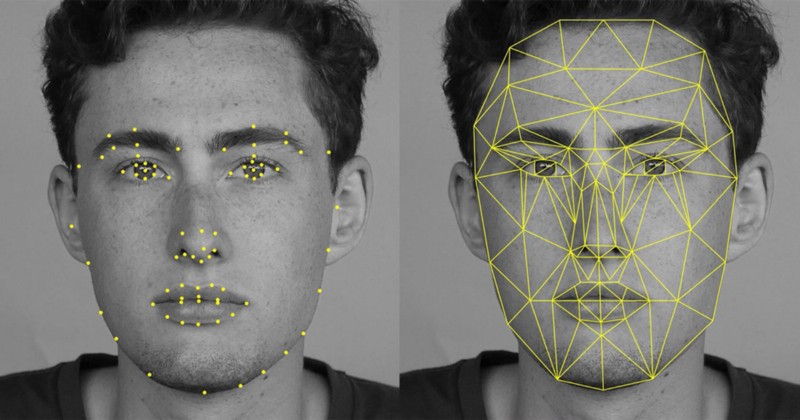
\includegraphics[width=\linewidth]{cnnFace.jpeg}
    \caption{Herkennen van features om zo een digitaal gezicht te maken}
    \label{fig:cnnface}
\end{figure}

\section{Degrees Of Freedom}

VR technologieën kunnen ook nog eens worden onderverdeeld afhankelijk van het aantal vrijheidsgraden dat ze ondersteunen. In de wereld van VR komen 3DOF en 6DOF het meeste voor. Deze vrijheidsgraden bepalen in welke mate de gebruiker kan bewegen in de virtuele wereld \autocite{Shenchang1995}.

% TODO TRANSLATE yaw, pitch, rol
3DOF ondersteund alleen rotationele bewegingen, deze zijn: yaw, pitch en rol. Hiermee kan camera alleen maar worden gedraaid en niet van locatie veranderen. Bij 6DOF zijn is dit wel mogelijk omdat deze over volgende bewegingen beschikt: up and down, front and back en left and right. 
Wanneer 6DOF wordt gebruikt kan er dus in de virtuele wereld worden rondgelopen alsook kan de camera nog steeds worden gedraaid omdat 6DOF beschikt over rotationale en positionele bewegingen, de ondersteuning van deze vrijheidsgraden ligt niet alleen bij de technologie zelf maar ook bij de gebruikte hardware \autocite{Shenchang1995}. In de longlist zal er in detail worden besproken hoeveel vrijheidsgraden ondersteund worden en welke hardware er juist nodig is om te gebruiken.

\begin{figure}
    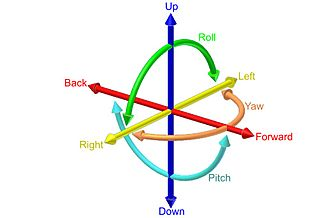
\includegraphics[width=\linewidth]{dof.jpg}
    \caption{Six degrees of freedom}
    \label{fig:dof}
\end{figure}

\section{Gelijkaardige use cases}
% TODO CONTENT Gelijkaardige use case
% TODO ASK Plaatsen na computer vision? Maakt gebruik van image scanning.
\subsection{Cleveland Museum of Art}
Dit museum maakt gebruik van software genaamd ArtLens. Artlens bestaat uit verschillende onderdelen die worden gecombineerd in 1 dezelfde smartphone app. Met deze app kunnen bezoekers een interactieve tour krijgen. In het museum bevinden zich bluetooth beacons waardoor de app kan weten waar de bezoeker zich bevind en zo tonen waar het volgende kunstwerk is. Ook kan de gebruiker zijn interesses opgeven waardoor de app voorstellen kan doen van kunstwerken die dichtbij zijn. 
De bezoekers kunnen ook zelf hun eigen tours maken en deze delen met andere gebruikers wat dan weer het sociale aspect van de applicatie bevordert.

Het VR gedeelte van deze applicatie vindt plaats wanneer een gebruiker met zijn camera op een schilderij mikt. Hierbij zal er dan op het scherm, via augmented reality, extra informatie komen over het schilderij.
In het museum bevinden zich ook terminals waar de gebruikers hun smartphone op kunnen leggen. Hierdoor verschijnt er op een groot scherm een opdracht die dan moet worden uitgevoerd bijvoorbeeld het nadoen van een schilderij of na een tijdje het schilderij zo goed mogelijk proberen natekenen \autocite{Ding2017}.

\subsection{Smithsonian}
Bij het Smithsonian wordt er ook gebruik gemaakt augmented reality, deze keer door gebruik te maken van BroadcastAR. Deze software gebruikt een camera om zo te streamen naar een groot scherm waarop de AR-objecten dan worden getoond. Het nadeel van deze implementatie is dat er weinig of geen interactie is tussen de gebruiker en de software. 

Het Smithsonian heeft ook nog een tweede augemented reality app waarbij gebruikers hun camera kunnen richten op skeletten om zo het skelet om te toveren naar een model van het levend dier.

\subsection{Historium Brugge}
Het Historium in Brugge maakt geen gebruik van augemented reality maar wel van virtual reality. Er zijn 2 soorten ervaringen die worden aangeboden, City VR en Historium VR. Bij City VR kan de gebruiker verschillende locaties van Brugge bezoeken in VR terwijl hij bij Historium VR een interactive rondeleiding krijgt over het middeleeuwse Brugge. De City VR applicatie kan worden geïnstalleerd op elke smartphone die AR ondersteund voor Historium VR is er echter wel een VR headset inclusief controllers nodig. 

% \lipsum[7-20]
